\documentclass[10pt]{article}
\usepackage[a4paper, left=1.5cm, right=1.5cm, top=3.5cm]{geometry}
\usepackage[]{graphicx}
\usepackage{multicol}
\usepackage{amssymb}
\usepackage{titlesec}
\usepackage{wrapfig}
\usepackage{blindtext}
\usepackage{lipsum}
\usepackage{caption}
\usepackage{listings}
\usepackage{fancyhdr}
\usepackage{nopageno}
\usepackage{authblk}
\usepackage{amsmath} % tons of math stuff
\usepackage{mathtools} % e.g. alignment within matrix
\usepackage{bm} % provides shorthand for bold in math mode
\usepackage{esdiff} % provides derivative commands
\usepackage{xcolor}
\usepackage{csquotes} % e.g. provides \enquote
\fancyhf[]{}

% own fig. env. for multicols
\newenvironment{Figure}
  {\par\medskip\noindent\minipage{\linewidth}}
  {\endminipage\par\medskip}

\begin{titlepage}
    \title{Lattice QCD}
    \author[1]{Angelo V. Brade\thanks{s72abrad@uni-bonn.de}}
    \affil[1]{Rheinische Friedrich-Wilhelms-Universität Bonn}
    \date{\today}
\end{titlepage}

\begin{document}
\pagenumbering{gobble}
\maketitle
\newpage

\tableofcontents
\newpage

\pagenumbering{arabic}

\pagestyle{fancy}
\fancyhead[R]{\thepage}
\fancyhead[L]{\leftmark}



\section{p2gg}
\subsection{Lower bound}
\begin{Figure}
  \centering\resizebox{\textwidth}{!}{% GNUPLOT: LaTeX picture with Postscript
\begingroup
  \makeatletter
  \providecommand\color[2][]{%
    \GenericError{(gnuplot) \space\space\space\@spaces}{%
      Package color not loaded in conjunction with
      terminal option `colourtext'%
    }{See the gnuplot documentation for explanation.%
    }{Either use 'blacktext' in gnuplot or load the package
      color.sty in LaTeX.}%
    \renewcommand\color[2][]{}%
  }%
  \providecommand\includegraphics[2][]{%
    \GenericError{(gnuplot) \space\space\space\@spaces}{%
      Package graphicx or graphics not loaded%
    }{See the gnuplot documentation for explanation.%
    }{The gnuplot epslatex terminal needs graphicx.sty or graphics.sty.}%
    \renewcommand\includegraphics[2][]{}%
  }%
  \providecommand\rotatebox[2]{#2}%
  \@ifundefined{ifGPcolor}{%
    \newif\ifGPcolor
    \GPcolortrue
  }{}%
  \@ifundefined{ifGPblacktext}{%
    \newif\ifGPblacktext
    \GPblacktexttrue
  }{}%
  % define a \g@addto@macro without @ in the name:
  \let\gplgaddtomacro\g@addto@macro
  % define empty templates for all commands taking text:
  \gdef\gplbacktext{}%
  \gdef\gplfronttext{}%
  \makeatother
  \ifGPblacktext
    % no textcolor at all
    \def\colorrgb#1{}%
    \def\colorgray#1{}%
  \else
    % gray or color?
    \ifGPcolor
      \def\colorrgb#1{\color[rgb]{#1}}%
      \def\colorgray#1{\color[gray]{#1}}%
      \expandafter\def\csname LTw\endcsname{\color{white}}%
      \expandafter\def\csname LTb\endcsname{\color{black}}%
      \expandafter\def\csname LTa\endcsname{\color{black}}%
      \expandafter\def\csname LT0\endcsname{\color[rgb]{1,0,0}}%
      \expandafter\def\csname LT1\endcsname{\color[rgb]{0,1,0}}%
      \expandafter\def\csname LT2\endcsname{\color[rgb]{0,0,1}}%
      \expandafter\def\csname LT3\endcsname{\color[rgb]{1,0,1}}%
      \expandafter\def\csname LT4\endcsname{\color[rgb]{0,1,1}}%
      \expandafter\def\csname LT5\endcsname{\color[rgb]{1,1,0}}%
      \expandafter\def\csname LT6\endcsname{\color[rgb]{0,0,0}}%
      \expandafter\def\csname LT7\endcsname{\color[rgb]{1,0.3,0}}%
      \expandafter\def\csname LT8\endcsname{\color[rgb]{0.5,0.5,0.5}}%
    \else
      % gray
      \def\colorrgb#1{\color{black}}%
      \def\colorgray#1{\color[gray]{#1}}%
      \expandafter\def\csname LTw\endcsname{\color{white}}%
      \expandafter\def\csname LTb\endcsname{\color{black}}%
      \expandafter\def\csname LTa\endcsname{\color{black}}%
      \expandafter\def\csname LT0\endcsname{\color{black}}%
      \expandafter\def\csname LT1\endcsname{\color{black}}%
      \expandafter\def\csname LT2\endcsname{\color{black}}%
      \expandafter\def\csname LT3\endcsname{\color{black}}%
      \expandafter\def\csname LT4\endcsname{\color{black}}%
      \expandafter\def\csname LT5\endcsname{\color{black}}%
      \expandafter\def\csname LT6\endcsname{\color{black}}%
      \expandafter\def\csname LT7\endcsname{\color{black}}%
      \expandafter\def\csname LT8\endcsname{\color{black}}%
    \fi
  \fi
    \setlength{\unitlength}{0.0500bp}%
    \ifx\gptboxheight\undefined%
      \newlength{\gptboxheight}%
      \newlength{\gptboxwidth}%
      \newsavebox{\gptboxtext}%
    \fi%
    \setlength{\fboxrule}{0.5pt}%
    \setlength{\fboxsep}{1pt}%
    \definecolor{tbcol}{rgb}{1,1,1}%
\begin{picture}(7200.00,4320.00)%
    \gplgaddtomacro\gplbacktext{%
      \csname LTb\endcsname%%
      \put(634,619){\makebox(0,0)[r]{\strut{}$1$}}%
      \csname LTb\endcsname%%
      \put(634,1006){\makebox(0,0)[r]{\strut{}$1.2$}}%
      \csname LTb\endcsname%%
      \put(634,1394){\makebox(0,0)[r]{\strut{}$1.4$}}%
      \csname LTb\endcsname%%
      \put(634,1781){\makebox(0,0)[r]{\strut{}$1.6$}}%
      \csname LTb\endcsname%%
      \put(634,2169){\makebox(0,0)[r]{\strut{}$1.8$}}%
      \csname LTb\endcsname%%
      \put(634,2556){\makebox(0,0)[r]{\strut{}$2$}}%
      \csname LTb\endcsname%%
      \put(634,2944){\makebox(0,0)[r]{\strut{}$2.2$}}%
      \csname LTb\endcsname%%
      \put(634,3331){\makebox(0,0)[r]{\strut{}$2.4$}}%
      \csname LTb\endcsname%%
      \put(634,3719){\makebox(0,0)[r]{\strut{}$2.6$}}%
      \csname LTb\endcsname%%
      \put(1513,425){\makebox(0,0){\strut{}$20$}}%
      \csname LTb\endcsname%%
      \put(2490,425){\makebox(0,0){\strut{}$30$}}%
      \csname LTb\endcsname%%
      \put(3467,425){\makebox(0,0){\strut{}$40$}}%
      \csname LTb\endcsname%%
      \put(4444,425){\makebox(0,0){\strut{}$50$}}%
      \csname LTb\endcsname%%
      \put(5420,425){\makebox(0,0){\strut{}$60$}}%
      \csname LTb\endcsname%%
      \put(6397,425){\makebox(0,0){\strut{}$70$}}%
    }%
    \gplgaddtomacro\gplfronttext{%
      \csname LTb\endcsname%%
      \put(6123,3545){\makebox(0,0)[r]{\strut{}$\chi^2$}}%
      \csname LTb\endcsname%%
      \put(170,2169){\rotatebox{-270.00}{\makebox(0,0){\strut{}$\log_e[\chi^2/2]$}}}%
      \csname LTb\endcsname%%
      \put(3809,135){\makebox(0,0){\strut{}$t_{\text{lower}}$}}%
      \csname LTb\endcsname%%
      \put(3809,4009){\makebox(0,0){\strut{}Lower bound}}%
    }%
    \gplbacktext
    \put(0,0){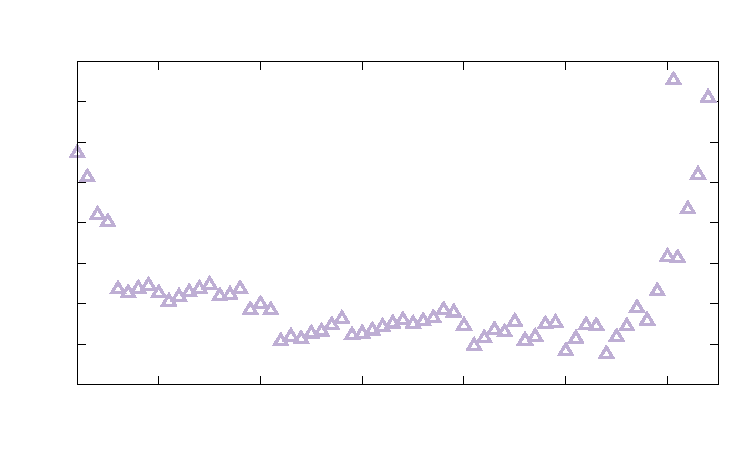
\includegraphics[width={360.00bp},height={216.00bp}]{LowerBound}}%
    \gplfronttext
  \end{picture}%
\endgroup
}
  \captionof{figure}{
    Lower bound for stable correlations.
  }
  \label{fig:1.1}
\end{Figure}

%Es lässt sich erkennen, dass bei \(t_\text{lower}=5\) der Fehler \(\Delta E\) am geringsten ist. Somit werden fortan all vorherien abgeschnitten.

\subsection{Upper bound}
\begin{Figure}
  \centering\resizebox{\textwidth}{!}{% GNUPLOT: LaTeX picture with Postscript
\begingroup
  \makeatletter
  \providecommand\color[2][]{%
    \GenericError{(gnuplot) \space\space\space\@spaces}{%
      Package color not loaded in conjunction with
      terminal option `colourtext'%
    }{See the gnuplot documentation for explanation.%
    }{Either use 'blacktext' in gnuplot or load the package
      color.sty in LaTeX.}%
    \renewcommand\color[2][]{}%
  }%
  \providecommand\includegraphics[2][]{%
    \GenericError{(gnuplot) \space\space\space\@spaces}{%
      Package graphicx or graphics not loaded%
    }{See the gnuplot documentation for explanation.%
    }{The gnuplot epslatex terminal needs graphicx.sty or graphics.sty.}%
    \renewcommand\includegraphics[2][]{}%
  }%
  \providecommand\rotatebox[2]{#2}%
  \@ifundefined{ifGPcolor}{%
    \newif\ifGPcolor
    \GPcolortrue
  }{}%
  \@ifundefined{ifGPblacktext}{%
    \newif\ifGPblacktext
    \GPblacktexttrue
  }{}%
  % define a \g@addto@macro without @ in the name:
  \let\gplgaddtomacro\g@addto@macro
  % define empty templates for all commands taking text:
  \gdef\gplbacktext{}%
  \gdef\gplfronttext{}%
  \makeatother
  \ifGPblacktext
    % no textcolor at all
    \def\colorrgb#1{}%
    \def\colorgray#1{}%
  \else
    % gray or color?
    \ifGPcolor
      \def\colorrgb#1{\color[rgb]{#1}}%
      \def\colorgray#1{\color[gray]{#1}}%
      \expandafter\def\csname LTw\endcsname{\color{white}}%
      \expandafter\def\csname LTb\endcsname{\color{black}}%
      \expandafter\def\csname LTa\endcsname{\color{black}}%
      \expandafter\def\csname LT0\endcsname{\color[rgb]{1,0,0}}%
      \expandafter\def\csname LT1\endcsname{\color[rgb]{0,1,0}}%
      \expandafter\def\csname LT2\endcsname{\color[rgb]{0,0,1}}%
      \expandafter\def\csname LT3\endcsname{\color[rgb]{1,0,1}}%
      \expandafter\def\csname LT4\endcsname{\color[rgb]{0,1,1}}%
      \expandafter\def\csname LT5\endcsname{\color[rgb]{1,1,0}}%
      \expandafter\def\csname LT6\endcsname{\color[rgb]{0,0,0}}%
      \expandafter\def\csname LT7\endcsname{\color[rgb]{1,0.3,0}}%
      \expandafter\def\csname LT8\endcsname{\color[rgb]{0.5,0.5,0.5}}%
    \else
      % gray
      \def\colorrgb#1{\color{black}}%
      \def\colorgray#1{\color[gray]{#1}}%
      \expandafter\def\csname LTw\endcsname{\color{white}}%
      \expandafter\def\csname LTb\endcsname{\color{black}}%
      \expandafter\def\csname LTa\endcsname{\color{black}}%
      \expandafter\def\csname LT0\endcsname{\color{black}}%
      \expandafter\def\csname LT1\endcsname{\color{black}}%
      \expandafter\def\csname LT2\endcsname{\color{black}}%
      \expandafter\def\csname LT3\endcsname{\color{black}}%
      \expandafter\def\csname LT4\endcsname{\color{black}}%
      \expandafter\def\csname LT5\endcsname{\color{black}}%
      \expandafter\def\csname LT6\endcsname{\color{black}}%
      \expandafter\def\csname LT7\endcsname{\color{black}}%
      \expandafter\def\csname LT8\endcsname{\color{black}}%
    \fi
  \fi
    \setlength{\unitlength}{0.0500bp}%
    \ifx\gptboxheight\undefined%
      \newlength{\gptboxheight}%
      \newlength{\gptboxwidth}%
      \newsavebox{\gptboxtext}%
    \fi%
    \setlength{\fboxrule}{0.5pt}%
    \setlength{\fboxsep}{1pt}%
    \definecolor{tbcol}{rgb}{1,1,1}%
\begin{picture}(7200.00,4320.00)%
    \gplgaddtomacro\gplbacktext{%
      \csname LTb\endcsname%%
      \put(634,619){\makebox(0,0)[r]{\strut{}$0.7$}}%
      \csname LTb\endcsname%%
      \put(634,963){\makebox(0,0)[r]{\strut{}$0.8$}}%
      \csname LTb\endcsname%%
      \put(634,1308){\makebox(0,0)[r]{\strut{}$0.9$}}%
      \csname LTb\endcsname%%
      \put(634,1652){\makebox(0,0)[r]{\strut{}$1$}}%
      \csname LTb\endcsname%%
      \put(634,1997){\makebox(0,0)[r]{\strut{}$1.1$}}%
      \csname LTb\endcsname%%
      \put(634,2341){\makebox(0,0)[r]{\strut{}$1.2$}}%
      \csname LTb\endcsname%%
      \put(634,2686){\makebox(0,0)[r]{\strut{}$1.3$}}%
      \csname LTb\endcsname%%
      \put(634,3030){\makebox(0,0)[r]{\strut{}$1.4$}}%
      \csname LTb\endcsname%%
      \put(634,3374){\makebox(0,0)[r]{\strut{}$1.5$}}%
      \csname LTb\endcsname%%
      \put(634,3719){\makebox(0,0)[r]{\strut{}$1.6$}}%
      \csname LTb\endcsname%%
      \put(731,425){\makebox(0,0){\strut{}$30$}}%
      \csname LTb\endcsname%%
      \put(978,425){\makebox(0,0){\strut{}$32$}}%
      \csname LTb\endcsname%%
      \put(1224,425){\makebox(0,0){\strut{}$34$}}%
      \csname LTb\endcsname%%
      \put(1470,425){\makebox(0,0){\strut{}$36$}}%
      \csname LTb\endcsname%%
      \put(1716,425){\makebox(0,0){\strut{}$38$}}%
      \csname LTb\endcsname%%
      \put(1962,425){\makebox(0,0){\strut{}$40$}}%
      \csname LTb\endcsname%%
      \put(2208,425){\makebox(0,0){\strut{}$42$}}%
      \csname LTb\endcsname%%
      \put(2455,425){\makebox(0,0){\strut{}$44$}}%
      \csname LTb\endcsname%%
      \put(2701,425){\makebox(0,0){\strut{}$46$}}%
      \csname LTb\endcsname%%
      \put(2947,425){\makebox(0,0){\strut{}$48$}}%
      \csname LTb\endcsname%%
      \put(3193,425){\makebox(0,0){\strut{}$50$}}%
      \csname LTb\endcsname%%
      \put(3439,425){\makebox(0,0){\strut{}$52$}}%
      \csname LTb\endcsname%%
      \put(3686,425){\makebox(0,0){\strut{}$54$}}%
      \csname LTb\endcsname%%
      \put(3932,425){\makebox(0,0){\strut{}$56$}}%
      \csname LTb\endcsname%%
      \put(4178,425){\makebox(0,0){\strut{}$58$}}%
      \csname LTb\endcsname%%
      \put(4424,425){\makebox(0,0){\strut{}$60$}}%
      \csname LTb\endcsname%%
      \put(4670,425){\makebox(0,0){\strut{}$62$}}%
      \csname LTb\endcsname%%
      \put(4916,425){\makebox(0,0){\strut{}$64$}}%
      \csname LTb\endcsname%%
      \put(5163,425){\makebox(0,0){\strut{}$66$}}%
      \csname LTb\endcsname%%
      \put(5409,425){\makebox(0,0){\strut{}$68$}}%
      \csname LTb\endcsname%%
      \put(5655,425){\makebox(0,0){\strut{}$70$}}%
      \csname LTb\endcsname%%
      \put(5901,425){\makebox(0,0){\strut{}$72$}}%
      \csname LTb\endcsname%%
      \put(6147,425){\makebox(0,0){\strut{}$74$}}%
      \csname LTb\endcsname%%
      \put(6393,425){\makebox(0,0){\strut{}$76$}}%
      \csname LTb\endcsname%%
      \put(6640,425){\makebox(0,0){\strut{}$78$}}%
      \csname LTb\endcsname%%
      \put(6886,425){\makebox(0,0){\strut{}$80$}}%
    }%
    \gplgaddtomacro\gplfronttext{%
      \csname LTb\endcsname%%
      \put(6123,3545){\makebox(0,0)[r]{\strut{}$\chi^2$}}%
      \csname LTb\endcsname%%
      \put(170,2169){\rotatebox{-270.00}{\makebox(0,0){\strut{}$\chi^2/$dof}}}%
      \csname LTb\endcsname%%
      \put(3809,135){\makebox(0,0){\strut{}$t_{\text{upper}}$}}%
      \csname LTb\endcsname%%
      \put(3809,4009){\makebox(0,0){\strut{}Upper bound}}%
    }%
    \gplbacktext
    \put(0,0){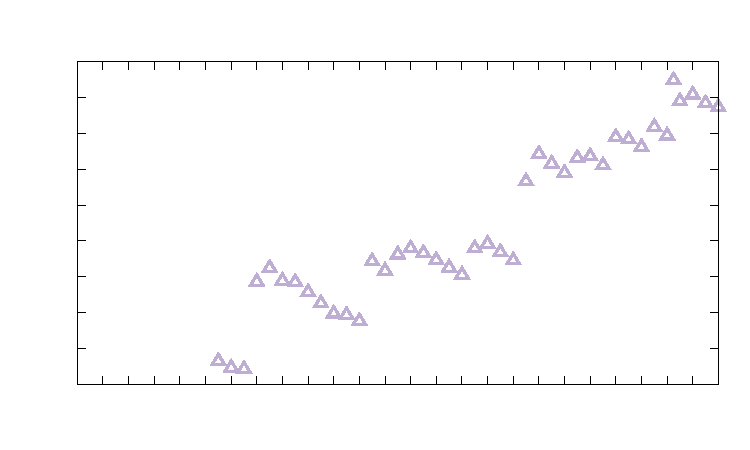
\includegraphics[width={360.00bp},height={216.00bp}]{UpperBound}}%
    \gplfronttext
  \end{picture}%
\endgroup
}
  \captionof{figure}{
    Upper bound for stable correlations.
  }
  \label{fig:1.2}

\subsection{Results}
\end{Figure}
\begin{Figure}
  \centering\resizebox{\textwidth}{!}{% GNUPLOT: LaTeX picture with Postscript
\begingroup
  \makeatletter
  \providecommand\color[2][]{%
    \GenericError{(gnuplot) \space\space\space\@spaces}{%
      Package color not loaded in conjunction with
      terminal option `colourtext'%
    }{See the gnuplot documentation for explanation.%
    }{Either use 'blacktext' in gnuplot or load the package
      color.sty in LaTeX.}%
    \renewcommand\color[2][]{}%
  }%
  \providecommand\includegraphics[2][]{%
    \GenericError{(gnuplot) \space\space\space\@spaces}{%
      Package graphicx or graphics not loaded%
    }{See the gnuplot documentation for explanation.%
    }{The gnuplot epslatex terminal needs graphicx.sty or graphics.sty.}%
    \renewcommand\includegraphics[2][]{}%
  }%
  \providecommand\rotatebox[2]{#2}%
  \@ifundefined{ifGPcolor}{%
    \newif\ifGPcolor
    \GPcolortrue
  }{}%
  \@ifundefined{ifGPblacktext}{%
    \newif\ifGPblacktext
    \GPblacktexttrue
  }{}%
  % define a \g@addto@macro without @ in the name:
  \let\gplgaddtomacro\g@addto@macro
  % define empty templates for all commands taking text:
  \gdef\gplbacktext{}%
  \gdef\gplfronttext{}%
  \makeatother
  \ifGPblacktext
    % no textcolor at all
    \def\colorrgb#1{}%
    \def\colorgray#1{}%
  \else
    % gray or color?
    \ifGPcolor
      \def\colorrgb#1{\color[rgb]{#1}}%
      \def\colorgray#1{\color[gray]{#1}}%
      \expandafter\def\csname LTw\endcsname{\color{white}}%
      \expandafter\def\csname LTb\endcsname{\color{black}}%
      \expandafter\def\csname LTa\endcsname{\color{black}}%
      \expandafter\def\csname LT0\endcsname{\color[rgb]{1,0,0}}%
      \expandafter\def\csname LT1\endcsname{\color[rgb]{0,1,0}}%
      \expandafter\def\csname LT2\endcsname{\color[rgb]{0,0,1}}%
      \expandafter\def\csname LT3\endcsname{\color[rgb]{1,0,1}}%
      \expandafter\def\csname LT4\endcsname{\color[rgb]{0,1,1}}%
      \expandafter\def\csname LT5\endcsname{\color[rgb]{1,1,0}}%
      \expandafter\def\csname LT6\endcsname{\color[rgb]{0,0,0}}%
      \expandafter\def\csname LT7\endcsname{\color[rgb]{1,0.3,0}}%
      \expandafter\def\csname LT8\endcsname{\color[rgb]{0.5,0.5,0.5}}%
    \else
      % gray
      \def\colorrgb#1{\color{black}}%
      \def\colorgray#1{\color[gray]{#1}}%
      \expandafter\def\csname LTw\endcsname{\color{white}}%
      \expandafter\def\csname LTb\endcsname{\color{black}}%
      \expandafter\def\csname LTa\endcsname{\color{black}}%
      \expandafter\def\csname LT0\endcsname{\color{black}}%
      \expandafter\def\csname LT1\endcsname{\color{black}}%
      \expandafter\def\csname LT2\endcsname{\color{black}}%
      \expandafter\def\csname LT3\endcsname{\color{black}}%
      \expandafter\def\csname LT4\endcsname{\color{black}}%
      \expandafter\def\csname LT5\endcsname{\color{black}}%
      \expandafter\def\csname LT6\endcsname{\color{black}}%
      \expandafter\def\csname LT7\endcsname{\color{black}}%
      \expandafter\def\csname LT8\endcsname{\color{black}}%
    \fi
  \fi
    \setlength{\unitlength}{0.0500bp}%
    \ifx\gptboxheight\undefined%
      \newlength{\gptboxheight}%
      \newlength{\gptboxwidth}%
      \newsavebox{\gptboxtext}%
    \fi%
    \setlength{\fboxrule}{0.5pt}%
    \setlength{\fboxsep}{1pt}%
    \definecolor{tbcol}{rgb}{1,1,1}%
\begin{picture}(7200.00,4320.00)%
    \gplgaddtomacro\gplbacktext{%
      \csname LTb\endcsname%%
      \put(1319,619){\makebox(0,0)[r]{\strut{}$0.00247875$}}%
      \csname LTb\endcsname%%
      \put(1319,2169){\makebox(0,0)[r]{\strut{}$0.00673795$}}%
      \csname LTb\endcsname%%
      \put(1319,3719){\makebox(0,0)[r]{\strut{}$0.0183156$}}%
      \csname LTb\endcsname%%
      \put(1759,425){\makebox(0,0){\strut{}$20$}}%
      \csname LTb\endcsname%%
      \put(2613,425){\makebox(0,0){\strut{}$30$}}%
      \csname LTb\endcsname%%
      \put(3468,425){\makebox(0,0){\strut{}$40$}}%
      \csname LTb\endcsname%%
      \put(4322,425){\makebox(0,0){\strut{}$50$}}%
      \csname LTb\endcsname%%
      \put(5177,425){\makebox(0,0){\strut{}$60$}}%
      \csname LTb\endcsname%%
      \put(6031,425){\makebox(0,0){\strut{}$70$}}%
      \csname LTb\endcsname%%
      \put(6886,425){\makebox(0,0){\strut{}$80$}}%
    }%
    \gplgaddtomacro\gplfronttext{%
      \csname LTb\endcsname%%
      \put(6123,3545){\makebox(0,0)[r]{\strut{}simulation data}}%
      \csname LTb\endcsname%%
      \put(6123,3351){\makebox(0,0)[r]{\strut{}fit curve with bootstrapping}}%
      \csname LTb\endcsname%%
      \put(170,2169){\rotatebox{-270.00}{\makebox(0,0){\strut{}$\langle x(0)x(\tau)\rangle$}}}%
      \csname LTb\endcsname%%
      \put(4151,135){\makebox(0,0){\strut{}$\tau$}}%
      \csname LTb\endcsname%%
      \put(4151,4009){\makebox(0,0){\strut{}Correlation function}}%
    }%
    \gplbacktext
    \put(0,0){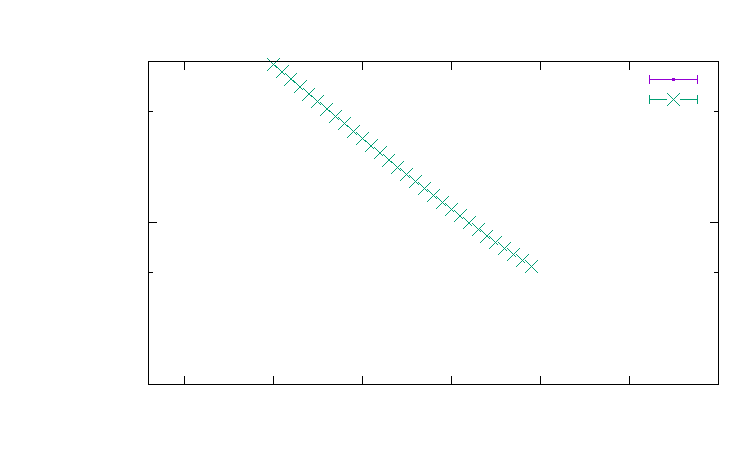
\includegraphics[width={360.00bp},height={216.00bp}]{CorrelationFunction}}%
    \gplfronttext
  \end{picture}%
\endgroup
}
  \captionof{figure}{
    Lower bound for stable correlations.
  }
  \label{fig:1.3}
\end{Figure}

Wir finden die in Tablle \ref{Tab:1.1} aufgeführten Werte, wobei die Correlatoren von \(t_\text{lower}=16\) und \(t_\text{upper}=80\) ausgewertet wurden, mit \(\chi^2=0.884\), \(X_0:=\) X ohne Bootstrapping, \(X_\text{boot.}:=\) X mit Bootstrapping, \(\frac{X_0 - X_\text{boot.}}{X_0}:=\) der normierten relativen Abweichung des Bootstrapps zu dem originalem Wert und \(\frac{\sigma_{X_\text{boot.}}}{X_0}:=\) dem normierten Fehler des Bootstrapps.

\begin{center}
\begin{tabular}{ccccccc}
  \(X\)&\(X_0\)&\(\sigma X_0\)&\(X_\text{boot.}\)&\(\sigma X_\text{boot.}\)&\(\frac{X_0 - X_\text{boot.}}{X_0}\)&\(\frac{\sigma_{X_\text{boot.}}}{X_0}\)\\
  \hline
  C & 3.3644e-03 & 1.7799e-05 & 3.3545e-03 & 2.1428e-05 & 2.9339e-03 & 6.3691e-03\\
  E & 4.7360e-02 & 3.9729e-05 & 4.7361e-02 & 4.3186e-05 & -2.0330e-05 & 9.1187e-04
\end{tabular}
\captionof{table}{Ergebnisse zur p2gg Auswertung.}
\label{Tab:1.1}
\end{center}


\end{document}
